\documentclass[a4paper,12pt,oneside]{book}

%-------------------------------Start of the Preable------------------------------------------------
\usepackage[english]{babel}
\usepackage{blindtext}
%packagr for hyperlinks
\usepackage{hyperref}
\hypersetup{
    colorlinks=true,
    linkcolor=blue,
    filecolor=magenta,      
    urlcolor=cyan,
}

\urlstyle{same}
%use of package fancy header
\usepackage{fancyhdr}
\setlength\headheight{26pt}
\fancyhf{}
%\rhead{
\includegraphics[width=1cm]{logo}}
\lhead{\rightmark}
\rhead{
\includegraphics[width=1cm]{logo}}
\fancyfoot[RE, RO]{\thepage}
\fancyfoot[CE, CO]{\href{http://www.e-yantra.org}{www.e-yantra.org}}

\pagestyle{fancy}

%use of package for section title formatting
\usepackage{titlesec}
\titleformat{\chapter}
  {\Large\bfseries} % format
  {}                % label
  {0pt}             % sep
  {\huge}           % before-code
 
%use of package tcolorbox for colorful textbox
\usepackage[most]{tcolorbox}
\tcbset{colback=cyan!5!white,colframe=cyan!75!black,halign title = flush center}

\newtcolorbox{mybox}[1]{colback=cyan!5!white,
colframe=cyan!75!black,fonttitle=\bfseries,
title=\textbf{\Large{#1}}}

%use of package marginnote for notes in margin
\usepackage{marginnote}

%use of packgage watermark for pages
%\usepackage{draftwatermark}
%\SetWatermarkText{
\includegraphics{logo}}
\usepackage[scale=2,opacity=0.1,angle=0]{background}
\backgroundsetup{
contents={
\includegraphics{logo}}
}

%use of newcommand for keywords color
\usepackage{xcolor}
\newcommand{\keyword}[1]{\textcolor{red}{\textbf{#1}}}

%package for inserting pictures
\usepackage{graphicx}

%package for highlighting
\usepackage{color,soul}

%new command for table
\newcommand{\head}[1]{\textnormal{\textbf{#1}}}


%----------------------End of the Preamble---------------------------------------


\begin{document}

%---------------------Title Page------------------------------------------------
\begin{titlepage}
\raggedright
{\Large eYSIP2016\\[1cm]}
{\Huge\scshape ANDROID APP DEVELOPMENT FOR FIREBIRD V \\[.1in]}
\vfill
\begin{flushright}
{\large INTERN: Jatin Mittal\\}
{\large MENTORS: Yogita Mali \\}
{\large Abhishek Singh \\}
{\large Sachin Gupta \\}
{\large Duration of Internship: $ 21/05/2016-10/07/2016 $ \\}
\end{flushright}

{\itshape 2016, e-Yantra Publication}
\end{titlepage}
%-------------------------------------------------------------------------------

\chapter[Project Tag]{Android app development for Firebird V}
\section*{Abstract}
	This project is all about bringing all the features of Firebird V on our finger tips through our Android phone. We are able to perform all the basic operations of our robot namely motion control(includes forward motion, backward motion, left rotation, right rotation), getting the readings of all the sensors(includes Sharp sensors, Proximity sensors and White line sensors), changing the velocity using our smart phones. We have achieved this communication with robot wirelessly with the help of bluetooth module.
\newpage
\subsection*{Objective}
    The objective of the project was to develop an Android app which can be used for motion control, velocity control and sensor monitoring of Firebird V robot.
	\vspace{1cm}
		\begin{center}
	\begin{tabular}{|c|p{2.5in}|c|}
		\hline
		\textbf{Task No.} & \qquad \qquad \qquad \qquad \textbf{Task} & \textbf{Deadline}\\
		\hline
		$1$ & Understand the basic concepts of Java and Android & 1 Days\\
		\hline
		$2$ & Make first Android App - Hello World & 2 Days\\
		\hline
		$3$ & Interface the Bluetooth module with Firebird V & 2 Days\\
		\hline
		$4$ & Review the previously developed code and understand it properly & 4 Days\\
		\hline
		$5$ & To modify the UI compeletely & 5 Days\\
		\hline
		$6$ & Testing the app thoroughly on various Android devices and
		also on various android versions & 3 Days\\
		\hline
		$7$ & Testing the app to run on various tablets & 2 Days\\
		\hline
	\end{tabular}
	\end{center}
\newpage
\subsection*{Completion status}
\begin{enumerate}
	 	\item \textbf{\large Installation and Study basics of Android:}
	 	\begin{itemize}
			\item Installed Android Studio in my computer to develop the Android app.
			\item Learned about Activity and its life cycle, Services, Intents:
			\begin{itemize}
				\item Activity- An Activity is an application component that provides a screen with which users can interact in order to do something, such as dial the phone, take a photo, send an email, or view a map. Each activity is given a window in which to draw its user interface. The window typically fills the screen, but may be smaller than the screen and float on top of other windows.\\
				To create an activity, you must create a subclass of Activity (or an existing subclass of it). In your subclass, you need to implement callback methods that the system calls when the activity transitions between various states of its life cycle, such as when the activity is being created, stopped, resumed, or destroyed. The two most important callback methods are onCreate() and onPause().
				\item Service- A Service is an application component that can perform long-running operations in the background and does not provide a user interface. Another application component can start a service and it will continue to run in the background even if the user switches to another application. Additionally, a component can bind to a service to interact with it and even perform interprocess communication (IPC). For example, a service might handle network transactions, play music, perform file I/O, or interact with a content provider, all from the background.
				
				\item Intent- Intent is an abstract description of an operation to be performed. It can be used with startActivity to launch an Activity, broadcastIntent to send it to any interested BroadcastReceiver components, and startService(Intent) or bindService(Intent, ServiceConnection, int) to communicate with a background Service. 
			\end{itemize}
		\end{itemize}
		\newpage
		\item \textbf{\large Made first Android App - Hello World} 
			\begin{figure}[h]
				\begin{center}
					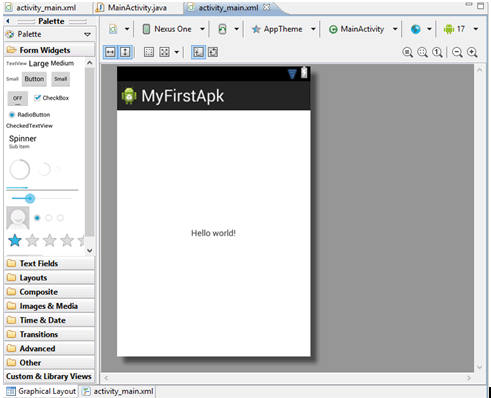
\includegraphics[scale=0.75]{helloworld.png}
				\end{center}
			\end{figure}
		\item \textbf{\large Developed UI for different activities}
		\begin{itemize}
		    	\item \textbf{Created Control Activity:}
		    	\begin{itemize}
		    	\item This is the first Activity that opens up when the app is launched.
				\item This Activity controls the forward, backward, left, right motion of the robot.
				\item It also contains the option to turn the buzzer on/off.
				\item TextView at the bottom of the Activity displays the current state of the buzzer.
				\item On clicking on the icon at the top right corner of the screen, a menu pops up which displays 'Connect' and 'Disconnect' option. 
				
				
			\end{itemize}
		    	\begin{figure}[h]
				    \begin{center}
					    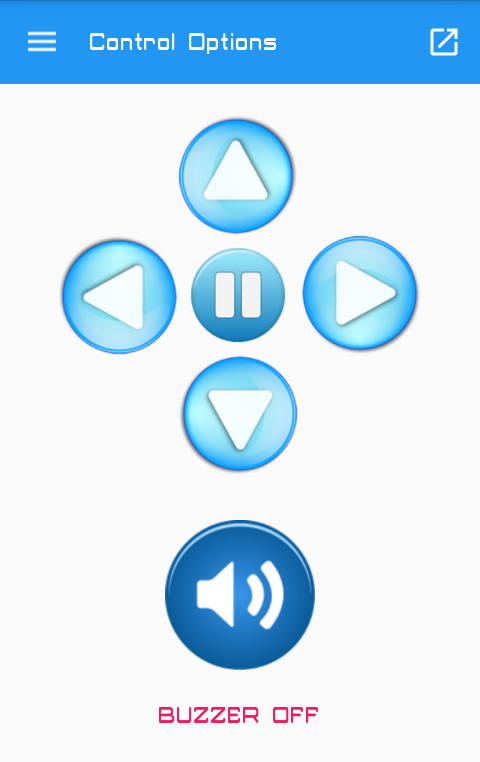
\includegraphics[scale=0.40]{control.png}
				    \end{center}
		    	\end{figure}
			
			\newpage
			\item \textbf{Created Drawer to navigate to other activities:}
			\begin{itemize}
				\item Navigation Drawer opens up when the icon at the top left corner of the screen is clicked.
				\item It allows us to navigate to other activities of the app.
				
			\end{itemize}
			
			\begin{figure}[h]
				\begin{center}
					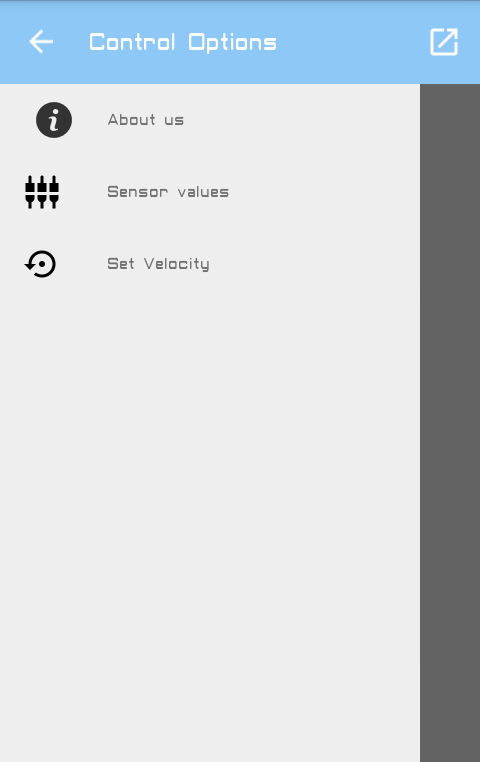
\includegraphics[scale=0.40]{drawer.png}
				\end{center}
			\end{figure}
			
			\newpage
			\item \textbf{Created Select Sensor Activity:}
			
			\begin{itemize}
				\item This Activity opens up when we select the 'Sensor Values' option from the drawer.
				\item This activity provides an option for Sharp sensor values, Proximity sensor values and White line sensor values.
			\end{itemize} 
			\begin{figure}[h]
				\begin{center}
					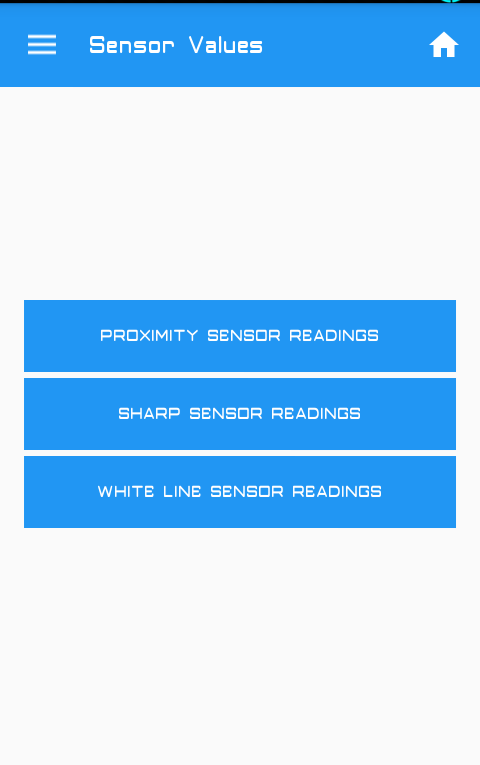
\includegraphics[scale=0.4]{selectsensor.png}
				\end{center}
			\end{figure}
			
			\newpage
			\item \textbf{Created Proximity Sensor Activity:}
			\begin{itemize}
				\item This Activity contains the bot image which shows the position of different proximity sensors on the bot.
				\item Below the image, there is a bar graph which displays the proximity sensor values.
				\item Values of the sensors can be updated by tapping on the chart.
			\end{itemize}
			\begin{figure}[h]
					\begin{center}
						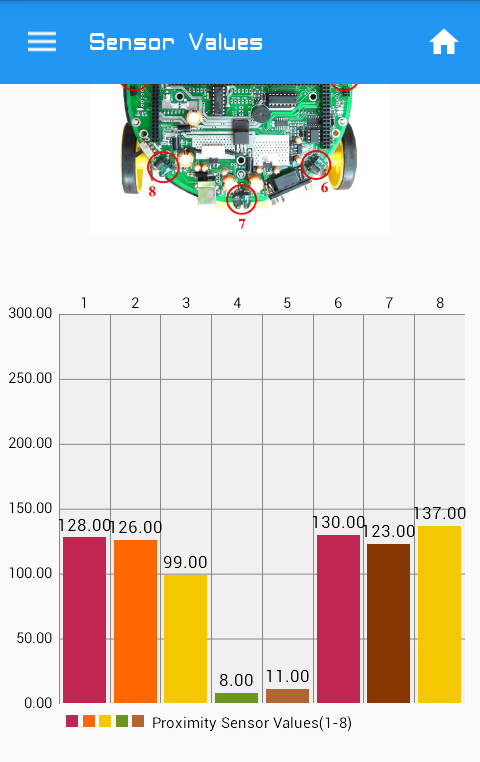
\includegraphics[scale=0.4]{proximitysensor.png}
					\end{center}
				\end{figure}
			\newpage    
			\item \textbf{Created Sharp Sensor Activity:}
			\begin{itemize}
				\item This Activity contains the bot image which shows the position of different Sharp sensors on the bot.
				\item Below the image, there is a bar graph which displays the Sharp sensor values.
				\item Values of the sensors can be updated by tapping on the chart.
			\end{itemize} 
				\begin{figure}[h]
					\begin{center}
						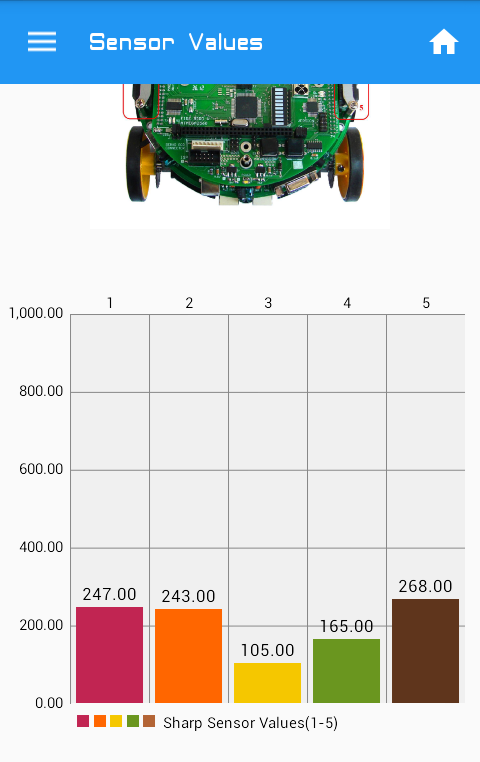
\includegraphics[scale=0.4]{sharpsensor.png}
					\end{center}
				\end{figure}
			\newpage
			\item \textbf{Created White Line Sensor Activity:}
			\begin{itemize}
			    \item This Activity contains the bot image which shows the position of different White line sensors on the bot.
				\item Below the image, there is a bar graph which displays the White line sensor values.
				\item Values of the sensors can be updated by tapping on the chart.
			\end{itemize}   	
			\begin{figure}[h]
				\begin{center}
				    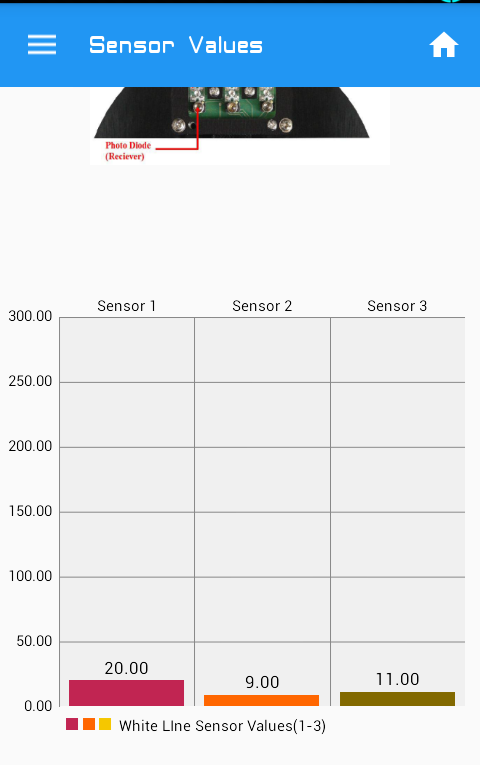
\includegraphics[scale=0.4]{whitelinesensor.png}
				\end{center}
			\end{figure} 
				
			\newpage
			\item \textbf{Created Set Velocity Activity:} 
			\begin{itemize}
			    \item This Activity opens up when we click on the 'Set Velocity' option in the drawer.
			    \item It contains two circular seekbar to set the velocities of left and right motor of the bot.
			    \item Below the sekkbars, there are TextView which displays the velocity value.
			    \item On clicking on the set button, the choosen velocity is set and the Control Activity is launched where we can control the bot motion with the velocity that we set.
			\end{itemize}
				\begin{figure}[h]
					\begin{center}
						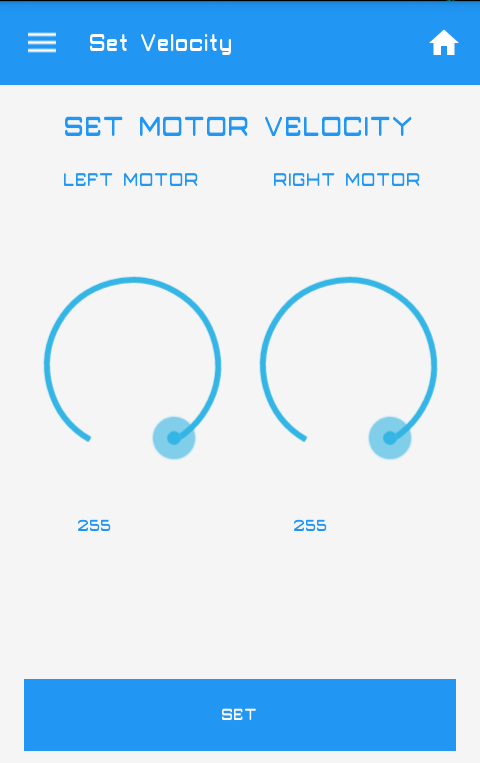
\includegraphics[scale=0.4]{setvelocity.png}
					\end{center}
				\end{figure}
		\end{itemize}	
		 \newpage
		\item \textbf{\large Testing} 
		    \begin{itemize}
			    \item Tested the app thoroughly on various Android devices and different versions of Android.
			    \item Tested the app on various tablets.
		    \end{itemize}
	\end{enumerate}
	\subsection*{Pending Task}
	    Adding the content in 'About Us' Activity is left.
	
		\\
    \subsection*{Hardware used}
		\begin{itemize}
		    \item Firebird V Robot 
            \item BlueLINK - bluetooth module
            \item Android Device
            \item 
            \href{./datasheet/AtMega2560.pdf}{Firebird V Robot - Datasheet}
            \item
            \href{http://www.nex-robotics.com/products/fire-bird-v-robots/fire-bird-v-atmega2560-robotic-research-platform.html}{Firebird V Robot - Vendor link}
            \item 
            \href{./datasheet/BlueLINK_External_Commands.pdf}{BlueLINK - Datasheet}
            \item 
            \href{https://www.rhydolabz.com/wiki/?tag=bluelink}{BlueLINK - Vendor link}
        \end{itemize}
        
    \subsection*{Software used}
        \begin{itemize}
            \item Android Studio v2.1.2  - 
             \href{https://developer.android.com/studio/index.html}{Download}
             \item Java SE Development Kit 8 - 
             \href{http://www.oracle.com/technetwork/java/javase/downloads/jdk8-downloads-2133151.html}{Downlaod}
            \item 
            \href {https://developer.android.com/studio/install.html}{Installation steps}
        \end{itemize}
    \subsection*{Software and code}
        \begin{itemize}
        \item Code : 
        \href{https://github.com/eYSIP-2016/Firebird_V_Testing_Android_App/tree/Wi-bird-App}{Github link} 
        \end{itemize}
	
	\subsection*{Use and demo}
    This is an Android Application to perform the basic testing of Firebird V robot. This application can be use to control the forward, backward, left, right motion of the bot, turning the buzzer on/off, setting the velocity of both the motors of the bot, and getting the different sensor values.\\
    
    \head{Use the following steps to test the Firebird V : }
    \begin{enumerate}
    \item First, turn on the Firebird V robot and pair the Android device to the Firebird V bluetooth by going into the bluetooth option of your phone.  
    \item Set the pin as 8888 for establishing the connection with the bot.
    \item Once the devices are paired, launch the application and select the device name from the paired devices list which is displayed on the screen.
    \item After the connection is established, test the bot by clicking on different buttons on the screen. This includes forward, backward, left, right motion, turning buzzer on/off.
    \item Motion of the bot can also be tested with different velocity of the bot. Open up the drawer and select the 'Set Velocity' option to set the different velocity of the bot.
    \item For checking the different sensor values, click on the 'Sensor values' option from the drawer and click on one of the buttons from 'proximity sensor readings', 'sharp sensor readings', 'white line sensor readings' to get the corresponding sensor values.
    \item After done with the testing, move to the control option Activity and click on the disconnect option that appears on clicking the icon at the top right corner of the screen.
    
    \end{enumerate}

\subsection*{Future Work}
 \begin{itemize}
	 	\item In future work, the same project can be implemented with wifi module and USB cable instead of bluetooth module.
	 	\item And, the possibility of improving the UI is always there.
	 \end{itemize} 

\subsection*{Bug report and Challenges}
\begin{itemize}
    \item The major problem with bluetooth module is that as it is short range it takes time to connect with bluetooth of our phone.We should keep our phone nearer to it so that the connection can be established faster.One major problem is that if once the connection is lost then robot has to be switched off and turned on again in order to establish connection again.
	\item One more issue is that after the successful connection made with the bot, the Title bar in Control Activity updates the subtitle that the connection is made, but if we return back to the same activity from some other activity it does not displays the subtitle even if the connection is still there.
\end{itemize} 

\end{enumerate} 
\newpage
\section*{References}
\begin{itemize}
    \item \href {http://www.androidhive.info/}{http://www.androidhive.info/}
    \item \href {http://www.stackoverflow.com}{http://www.stackoverflow.com}
	\item \href {https://github.com/neild001/SeekArc}{https://github.com/neild001/SeekArc}
	\item \href {https://www.numetriclabz.com/android-bar-chart-using-mpandroidchart-library-tutorial/}{https://www.numetriclabz.com/android-bar-chart-using-mpandroidchart-library-tutorial/}
	\item \href {https://www.tutorialspoint.com}{https://www.tutorialspoint.com}
	\item \href {https://www.developer.android.com}{https://www.developer.android.com}
	\item \href {https://github.com/PhilJay/MPAndroidChart}{https://github.com/PhilJay/MPAndroidChart}
	\item \href {http://stackoverflow.com/questions/22038576/how-to-draw-bar-chart-and-also-pie-chart-in-android}{http://stackoverflow.com/questions/22038576/how-to-draw-bar-chart-and-also-pie-chart-in-android}
	\item \href {https://developer.android.com/training/implementing-navigation/nav-drawer.html}{https://developer.android.com/training/implementing-navigation/nav-drawer.html}
	\item \href {https://www.youtube.com/watch?v=h57QpXp2TRg}{https://www.youtube.com/watch?v=h57QpXp2TRg}
	\item \href {https://www.youtube.com/watch?v=hrlGVU8z7zc}{https://www.youtube.com/watch?v=hrlGVU8z7zc}
	\item \href {https://www.youtube.com/watch?v=pMO8EVkhJO8}{https://www.youtube.com/watch?v=pMO8EVkhJO8}
	\item \href {https://www.youtube.com/watch?v=4XfDDfa3rv8}{https://www.youtube.com/watch?v=4XfDDfa3rv8}
	\item \href {https://github.com/slidenerd/Material-Design-Test-App-DEPRECATED-}{https://github.com/slidenerd/Material-Design-Test-App-DEPRECATED-}
\end{itemize}




\end{document}

